\documentclass[varwidth=40cm]{standalone}
\usepackage{tikz}
\usepackage{style}

\def\tmax{10}

\begin{document}
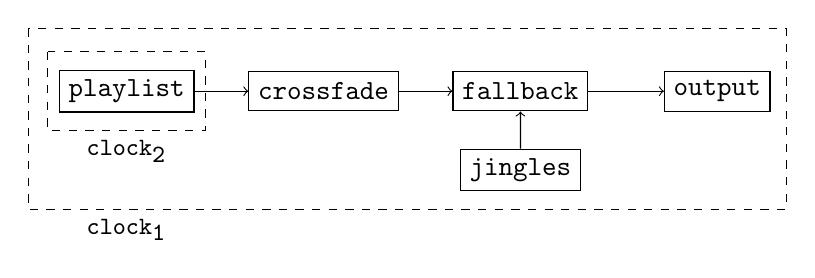
\begin{tikzpicture}[xscale=2.5,minimum size=5mm]
  \node[draw,shape=rectangle] (playlist) at (0,0) {\texttt{playlist}};
  \node[draw,shape=rectangle] (crossfade) at (1,0) {\texttt{crossfade}};
  \node[draw,shape=rectangle] (fallback) at (2,0) {\texttt{fallback}};
  \node[draw,shape=rectangle] (jingles) at (2,-1) {\texttt{jingles}};
  \node[draw,shape=rectangle] (output) at (3,0) {\texttt{output}};
  \draw[->] (playlist) edge (crossfade);
  \draw[->] (crossfade) edge (fallback);
  \draw[->] (jingles) edge (fallback);
  \draw[->] (fallback) edge (output);
  \draw[dashed] (-.4,.5) rectangle (.4,-.5);
  \draw[dashed] (-.5,.8) rectangle (3.35,-1.5);
  \draw (0,-.5) node[below] {\small$\texttt{clock}_{\texttt{2}}$};
  \draw (0,-1.5) node[below] {\small$\texttt{clock}_{\texttt{1}}$};
\end{tikzpicture}
\end{document}
